\section{Parallélisation avec OpenCL}

Dans cette partie nous verrons comment l'utilisation d'OpenCL permet d'améliorer les performances du programme par rapport au code séquentiel.

\paragraph{Résultats}
\begin{figure}[!h]
    \centering
    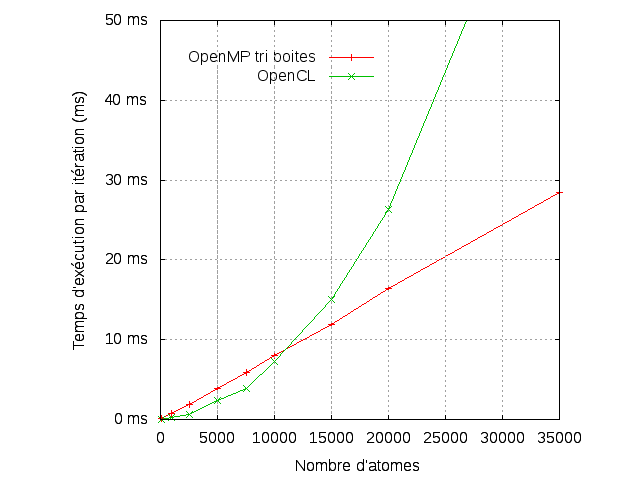
\includegraphics[scale=0.7]{./img/ocl.png}
    \caption{Comparatif OpenMP boites/OpenCL}
\end{figure}

Il est à noter que les performances obtenues avec OpenCL sont meilleures qu'avec OpenMP en considérant un nombre peu élevé d'atomes.
Mais cela est surtout dû à la puissance de calcul offerte par la carte graphique. L'algorithme utilisé pour la version OpenCL reste en $O(n^2)$ et n'optimise pas les calculs en fonction de la position des atomes, d'où les faibles performances comparées à la version OpenMP trié par boîte passé la barre des 10000 atomes. Cela dit, les performances restent bien meilleurs qu'avec la version non triée d'OpenMP.

Nous avons également pensé à une amélioration possible du code en créant au sein de chaque workgroup, un tableau de taille $TILE\_SIZE$. Chaque thread d'un workgroup s'occupe alors de charger les coordonnées d'un atome pour le ranger dans ce tableau. Une fois ce tableau rempli, on continue le calcul de la force, puis on charge un nouveau bloc de coordonnées, etc... Jusqu'à ce que tous les atomes soient parcourus. On divise ainsi le nombre d'accès aux coordonnées par la taille d'un workgroup. Cependant, en pratique, cela n'augmente pas les performances.